\section{Timing Performance Results from Calorimeter with SiPM Readout}
\label{sec:beamtiming}

Our previous results on precision timing with LYSO based calorimeters \cite{lysotiming} were obtained with multi-channel plate photo m
ultiplier (MCP-PMT) as photo detectors. MCP-PMTs feature a signal rise time on the order of 100 ps. For laser pulses with a FWHM of 50
 ps we achieved a differential timing resolution of 7 ps \cite{elba2015}, corresponding to a single device timing resolution of 5 ps. 
This performance is limited by the DRS based digitizer we use as a DAQ system, operating at 5 GS/s. In the studies described in this p
aper we use silicone multi pixel photon counters (SiPM).
While they feature a slower rise time they allow a very good timing performance for large, coherent signals \cite{aashrita}.  
For our setup we use four different types of SiPMs with 10, 15 and 25 $\mu$m pixel size and $1 \times 1$ mm and $3 \times 3$ mm sensor
 size \cite{hama}. They are all read out with a DRS based digitizer through a clipping circuit as described in \cite{aashrita}.
We do not amplify the output signal of the SiPMs, only exploiting the very large light yield of the LYSO scintillator and the intrinsi
c
amplification of the SiPMs.
Using the same fast laser pulses and DAQ system we obtain a differential timing resolution between two SiPMs of better than 10 ps, ver
y similar to the MCP-PMT performance.\\ 
The experimental setup we use for the calorimetric timing measurements consists of a single cell of a sampling calorimeter with 29 lay
ers of LYSO crystal and tungsten absorber. The lateral dimensions are $\mathrm{14 \times 14 \,mm^2}$. The total depth of the cell is a
bout 11.5 cm with the LYSO plates having a thickness of 1.5 mm. The scintillation light from the LYSO plates is extracted with four wa
ve length shifting (WLS) fibers. The same cell has been used to measure the timing performance in comparison to the timing performance
 of a single cube of LYSO \cite{lysotiming}. More details of the calorimetric performance of the Shashlik configuration are discussed 
in references \cite{shashlik1} and \cite{shashlik2}.\\
In addition to plastic WLS fibers we also tested quartz capillaries filled with liquid wave length shifter using DSB as a wave length 
shifting agent \cite{capillaries}. To optically couple the quartz capillaries to the SiPMs we use a clear plastic fiber light guide wh
ich is connected to the end of the quartz capillary with a metal sleave tube. The same clear fiber coupler is used for the plastic WLS
 fibers to maintain equivalent light collection efficiency. The ratio of the light collection efficiency between the plastic fibers an
d the quartz capillaries approximately scales with the ratio of the diameter of the plastic fiber and the liquid core of the quartz ca
pillary. This ratio is about 3 for the fibers and capillaries we used.\\  
As a timing reference we  use a Photek 240 MCP-PMT. It is placed behind the calorimeter cell and detects secondary shower particles es
caping from the Shashlik calorimeter cell as we did in our previous studies \cite{lysotiming}.
To extract the time of flight we measure the time difference between the reference counter and the calorimeter cell. The time stamp is
 extracted from a Gaussian fit to the peak of the reference counter pulse which resembles a Gaussian shape. For the time stamp from th
e calorimeter cell we perform a straight line fit to the rising edge of the pulse and extract the time at half of the maximal signal a
mplitude.\\
We measure the timing performance of the calorimeter cell with high energy electrons in a range between 20 GeV and 200 GeV in the CERN
 North Area test beam. The impact point of the electrons onto the calorimeter cell is measured with a fiber hodoscope with a precision
 of better than 1 mm. The timing results are extracted from events impacting in the center of the calorimeter cell in an area of 2x2 m
m. As we are using a single calorimeter cell the containment outside this region is limited which affects the timing measurement.\\


\section{Experimental Results}
The timing precision extracted from a pulse improves as the rise time of the pulse gets shorter and as the signal over background impr
oves. The rise time of the pulses from the shashlik calorimeter cell are driven by the time constants of the wave length shifter
as we demonstrated previously \cite{lysotiming}. The rise time of the LYSO scintillation signal and the rise time of the previously us
ed MCP-PMT is much faster than the WLS time constants.                                                                  
As SiPMs feature a slower rise time than MCP-PMTs we studied the signal rise time with our new setup.
In figure \ref{RiseTime} we show the rise time of the pulses as a function of the signal amplitude. 
%
\begin{figure}[htbc]
%\hspace*{-0.3cm}
%\begin{minipage}[b]{22pc}
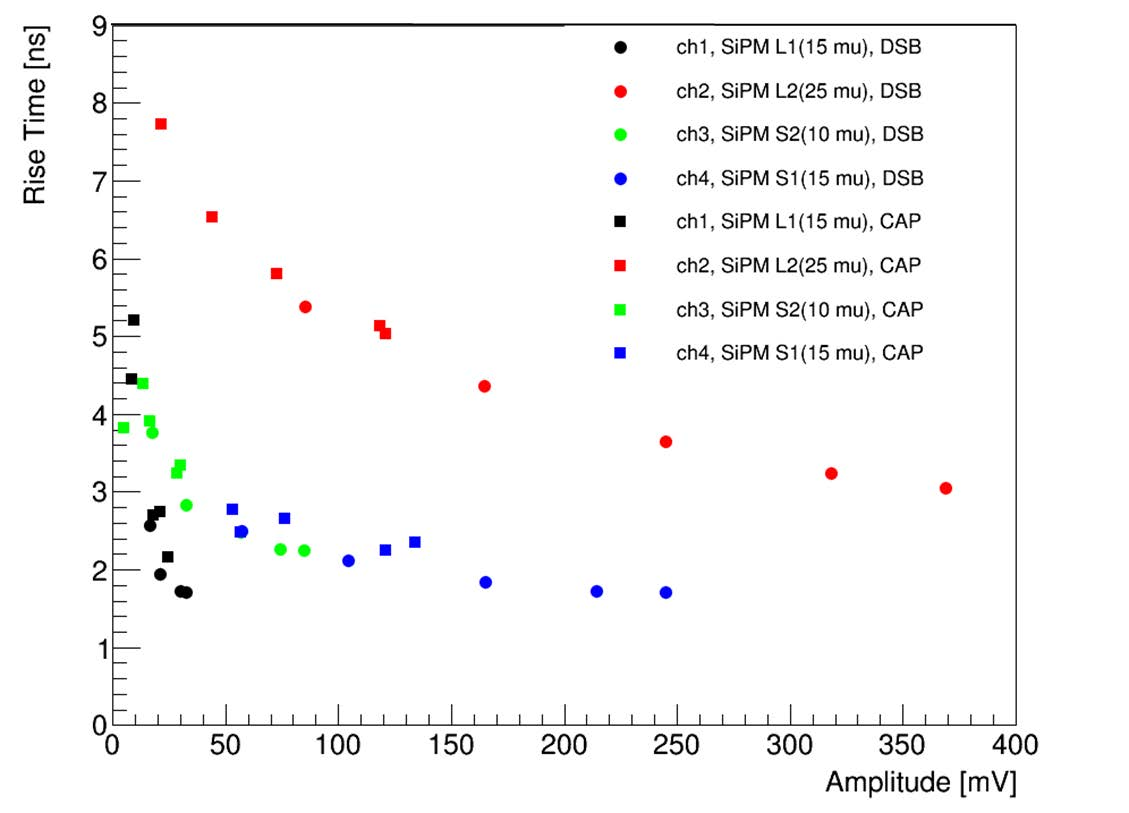
\includegraphics[width=0.99\textwidth]{RiseTime.pdf}
%\end{minipage}
%\begin{minipage}[b]{14pc}
\caption{\label{RiseTime}Rise time of the pulses as a function of the amplitude for the four different SiPMs.
 The data recorded with the plastic fibers and the quartz capillaries are distinguished as dots and squares. For each of the two data 
sets with plastic fibers and capillaries there are 5 measurements corresponding to beam energies of 20, 50, 100, 150 and 200 GeV.}
%\end{minipage}
%\hspace*{-0.3cm}
\end{figure}
%
We observe that the the rise time of the pulses becomes shorter for larger pulses, reaching around 2 ns for the largest amplitudes
in each channel. 
The amplitude dependency of the rise time is similar between different types of SiPMs but reaches is shortest value at
different signal amplitudes. 
The bias voltage of the SiPMs is set to the same voltage, no individual optimization has been
performed. The absolute signal amplitude in the SiPMs is different for the same beam energy which is expected as pixel count,
sensor size and the light guide coupling efficiency varies. The clipping circuit used for all SiPMs is the same while the capacitance 
of the  SiPMs is not.    
In figure \ref{TimeResolution} we show the time resolution of the four individual fibers as a function of their respective signal ampl
itude. Lines indicate the trend of the time resolution.
%
\begin{figure}[htbc]
%\hspace*{-0.3cm}
%\begin{minipage}[b]{22pc}
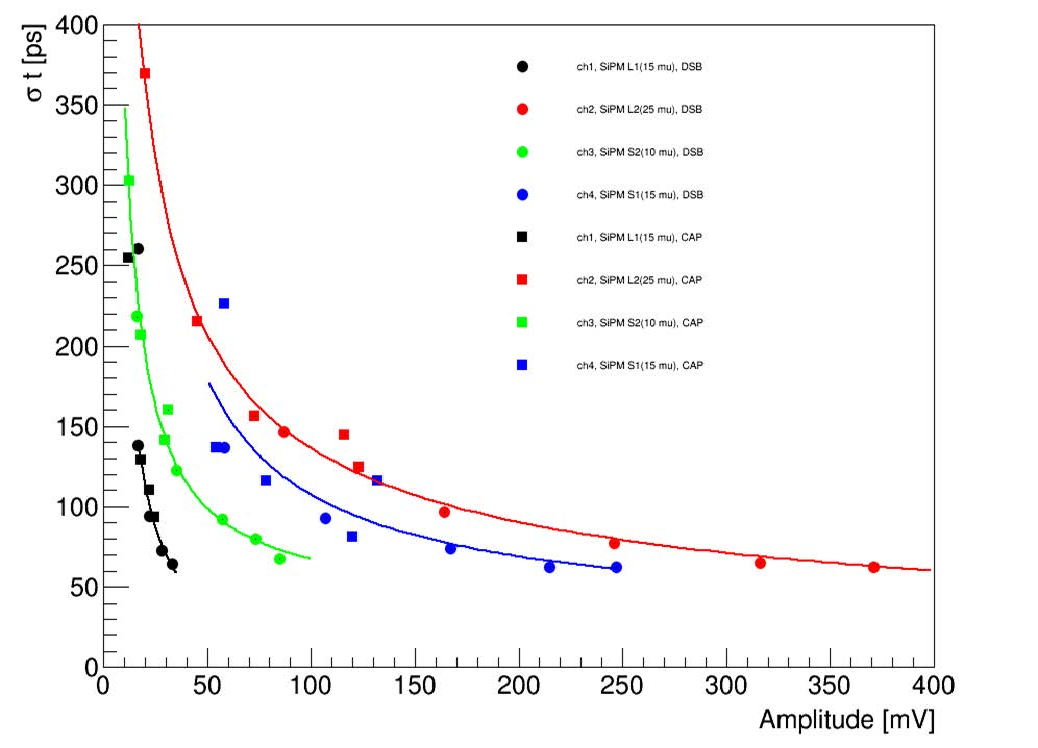
\includegraphics[width=0.99\textwidth]{SH_timing_SiPM.pdf}
%\end{minipage}
%\begin{minipage}[b]{14pc}
\caption{\label{TimeResolution} Time resolution achieved with the calorimeter cell using the signal of each o
f the  SiPMs individually. The data for each SiPM consists of two sets, one with the DSB WLS plastic fiber and one with the capillarie
s with a liquid DSB based WLS. The time resolution improves with increasing signal amplitude. The best time resolution per fibre is ar
ound 60 ps for all of the channels. The amplitude at which this performance is achieved varies.}
%\end{minipage}
%\hspace*{-0.3cm}
\end{figure}
%
We see a similar trend as for the rise times. However we also see
that the improvement of the timing resolution is not just due to the faster rise times.  
The increased signal amplitude and the resulting improvement in the signal over background results in additional improvement.

For the same amplitude we find the same timing resolution with the capillaries and the plastic WLS fibers, both using DSB WLS agent.
This further supports our previous findings that the the light propagation in the optical elements of a scintillation based calorimete
r dos not significantly affect the performance at the level of 50 ps.\\   
The light extraction efficiency of capillaries with liquid WLS remains sufficiently high for dose rates of 100 Mrad and beyond and for
 fluences of $\mathrm{10^{14} protons/cm^{2}}$ and beyond \cite{shashlik2}. The energy resolution performance of the LYSO/tungsten cel
l is not limited by photo statistics but the sampling fraction. The timing performance at lower energies could be improved by increasi
ng the raw signal. This could be achieved by using larger diameter capillaries.\\ 

